%%
%% This is file `sample-sigconf.tex',
%% generated with the docstrip utility.
%%
%% The original source files were:
%%
%% samples.dtx  (with options: `sigconf')
%% 
%% IMPORTANT NOTICE:
%% 
%% For the copyright see the source file.
%% 
%% Any modified versions of this file must be renamed
%% with new filenames distinct from sample-sigconf.tex.
%% 
%% For distribution of the original source see the terms
%% for copying and modification in the file samples.dtx.
%% 
%% This generated file may be distributed as long as the
%% original source files, as listed above, are part of the
%% same distribution. (The sources need not necessarily be
%% in the same archive or directory.)
%%
%% The first command in your LaTeX source must be the \documentclass command.
\documentclass[sigconf]{acmart}
\usepackage[ruled,vlined]{algorithm2e}
\usepackage{booktabs}
\usepackage{todonotes}
\SetKw{KwBy}{by}

%%
%% \BibTeX command to typeset BibTeX logo in the docs
\AtBeginDocument{%
  \providecommand\BibTeX{{%
    \normalfont B\kern-0.5em{\scshape i\kern-0.25em b}\kern-0.8em\TeX}}}

%% Rights management information.  This information is sent to you
%% when you complete the rights form.  These commands have SAMPLE
%% values in them; it is your responsibility as an author to replace
%% the commands and values with those provided to you when you
%% complete the rights form.
\setcopyright{acmcopyright}
\copyrightyear{2020}
\acmYear{2020}
\acmDOI{10.1145/1122445.1122456}

%% These commands are for a PROCEEDINGS abstract or paper.
\acmConference[MemSys '20]{MemSys 2020: The International Symposium on Memory Systems} {Sept 28--Oct 01, 2020}{Washington, DC}
%\acmBooktitle{MemSys '20: MemSys, Sept 28--Oct 01, 2020, Washington, DC}
\acmPrice{15.00}
\acmISBN{978-1-4503-XXXX-X/18/06}


%%
%% Submission ID.
%% Use this when submitting an article to a sponsored event. You'll
%% receive a unique submission ID from the organizers
%% of the event, and this ID should be used as the parameter to this command.
%%\acmSubmissionID{123-A56-BU3}

%%
%% The majority of ACM publications use numbered citations and
%% references.  The command \citestyle{authoryear} switches to the
%% "author year" style.
%%
%% If you are preparing content for an event
%% sponsored by ACM SIGGRAPH, you must use the "author year" style of
%% citations and references.
%% Uncommenting
%% the next command will enable that style.
%%\citestyle{acmauthoryear}

\begin{document}

%%
%% The "title" command has an optional parameter,
%% allowing the author to define a "short title" to be used in page headers.
\title{CircusTent: A Benchmark Suite for Atomic Memory Operations}

%%
%% The "author" command and its associated commands are used to define
%% the authors and their affiliations.
%% Of note is the shared affiliation of the first two authors, and the
%% "authornote" and "authornotemark" commands
%% used to denote shared contribution to the research.
\author{John D. Leidel}
\email{jleidel@tactcomplabs.com}
\orcid{0000-0002-7567-8145}
\affiliation{%
  \institution{Tactical Computing Laboratories}
  \city{Muenster}
  \state{Texas}
  \postcode{76252}
}

\author{Brody Williams}
\email{brody.williams@ttu.edu}
\affiliation{%A
  \institution{Texas Tech University}
  \city{Lubbock}
  \state{Texas}
  \postcode{79409-3104}
 }

\author{Xi Wang}
\email{xi.wang@ttu.edu}
\affiliation{%A
  \institution{Texas Tech University}
  \city{Lubbock}
  \state{Texas}
  \postcode{79409-3104}
}

\author{David Donofrio}
\email{ddonofrio@tactcomplabs.com}
\affiliation{%
  \institution{Tactical Computing Laboratories}
  \city{San Francisco}
  \state{California}
  \postcode{94102}
}

\author{Yong Chen}
\email{yong.chen@ttu.edu}
\affiliation{%A
  \institution{Texas Tech University}
  \city{Lubbock}
  \state{Texas}
  \postcode{79409-3104}
}

%%
%% By default, the full list of authors will be used in the page
%% headers. Often, this list is too long, and will overlap
%% other information printed in the page headers. This command allows
%% the author to define a more concise list
%% of authors' names for this purpose.
\renewcommand{\shortauthors}{Leidel and Williams, et al.}

% Abstract
\begin{abstract}
  A clear and well-documented \LaTeX\ document is presented as an
  article formatted for publication by ACM in a conference proceedings
  or journal publication. Based on the ``acmart'' document class, this
  article presents and explains many of the common variations, as well
  as many of the formatting elements an author may use in the
  preparation of the documentation of their work.
\end{abstract}

%%
%% The code below is generated by the tool at http://dl.acm.org/ccs.cfm.
%% Please copy and paste the code instead of the example below.
%%
%\begin{CCSXML}
%<ccs2012>
% <concept>
 % <concept_id>10010520.10010553.10010562</concept_id>
 % <concept_desc>Computer systems organization~Embedded systems</concept_desc>
 % <concept_significance>500</concept_significance>
 %</concept>
 %<concept>
 % <concept_id>10010520.10010575.10010755</concept_id>
 % <concept_desc>Computer systems organization~Redundancy</concept_desc>
 % <concept_significance>300</concept_significance>
 %</concept>
 %<concept>
  %<concept_id>10010520.10010553.10010554</concept_id>
  %<concept_desc>Computer systems organization~Robotics</concept_desc>
  %<concept_significance>100</concept_significance>
 %</concept>
 %<concept>
 % <concept_id>10003033.10003083.10003095</concept_id>
 % <concept_desc>Networks~Network reliability</concept_desc>
 % <concept_significance>100</concept_significance>
 %</concept>
%</ccs2012>
%\end{CCSXML}

%\ccsdesc[500]{Computer systems organization~Embedded systems}
%\ccsdesc[300]{Computer systems organization~Redundancy}
%\ccsdesc{Computer systems organization~Robotics}
%\ccsdesc[100]{Networks~Network reliability}

%%
%% Keywords. The author(s) should pick words that accurately describe
%% the work being presented. Separate the keywords with commas.
\keywords{benchmark, atomic memory operations, OpenMP, MPI, OpenSHMEM}

\maketitle

% Introduction
\section{Introduction}
\label{sec:introduction}
% Introduction Section

The impending demise of Moore's Law has produced a renaissance in the field of computer architecture.
Unable to continue leveraging increasing processor frequencies to further improve performance and scalability, system architects been have forced to explore other options.
In this new era of heterogeneous architectures and hardware/software codesign, parallel processing and associated programming paradigms have become of paramount importance.
Alongside an increased prominence in traditional high performance computing (HPC) environments in academia, government laboratories, and industry, parallel processing has also become imperative for consumer-level devices.
As such, a better understanding of the behavior of parallel applications, and their interaction with the architectures they run on, is highly desirable in order to ensure optimal performance.

One well understood characteristic of parallel applications is that they frequently suffer from scalability issues as the number of cooperating processing elements (PEs) grows.
Often, this performance degradation can be directly attributed to overheads associated with the synchronization of active PEs.
Consequently, well written applications utilize synchronization primitives, such as barriers and mutual exclusion locks, as infrequently as possible.
Regrettably, the nature of parallel applications typically precludes the removal of all such synchronization methods as they are necessary to prevent race conditions associated with access to shared data structures and ensure program correctness.
Given the impact synchronization plays on the scalability and performance of parallel applications, understanding and optimization of these routines is key.

In many cases, the synchronization primitives described above are constructed using atomic memory operations (AMOs).
Abstractly, an atomic memory operation can be defined as an operation that is uninterruptible.
Although an atomic operation may be composed of several smaller "sub-operations" that would, under other circumstances, necessitate the execution of multiple instructions to complete, herein these sub-operations are treated as a single, cohesive unit.
In this work, we focus on a particularly prominent class of atomic memory operations known as read-modify-write (RMW) atomics.
Most modern architectures, including x86, RISC-V, and those produced by ARM, include ISA-level RMW atomic instructions and provide microarchitectural support for realization of their execution.
As their designation would suggest, RMW atomics load a single value of a given data type into a specified register, modify said value, and finally write it back to memory in one unified step.
In this manner, RMW atomic operations can be utilized to safely set variables underlying more complex synchronization primitives, such as barriers and locks, in parallel environments.

Further, RMW atomics also constitute a particularly efficient and fine-grained synchronization primitive in and of themselves.
In many cases, application developers can replace mutex lock encapsulated critical code segments with "lock-free" atomic based synchronization.
Doing so allows parallel execution to continue to the greatest degree possible and often significantly improves application performance.
Many graph-based computational kernels, wherein only access to shared vertex and/or edge data need be coordinated, employ such an atomic-based synchronization scheme.
In our previous work, we examined the GAP Benchmark Suite, which is designed to replicate the memory access patterns of graph workloads in a shared memory environment, in order to quantify the proportion of atomic operations \cite{beamer2015gap}.
Therein, we found that, across all six included kernels, an average of 17.46\% of the total instructions were RMW atomic operation instructions \cite{rae}.
In this and similar scenarios, the frequency of atomic memory operations results in contention that, while less significant than lock-based synchronization, has measurable effects on application performance.

A variety of different shared and distributed memory parallel programming paradigms exist today in order to provide efficient scaling both within a single node, and across distinct nodes, respectively.
Unsurprisingly, variants of high-level synchronization constructs and atomic memory operations are critical for physically shared memory paradigms as well as distributed memory paradigms that utilize a shared memory abstraction.
For models designed specifically for physically shared memory systems, such as OpenMP or Pthreads, high-level synchronization primitives and API level atomic operations can be realized through simple wrappers around the appropriate ISA-level atomic instructions.
However, for distributed shared memory parallel programming models, the implementation of "remote atomics" and associated synchronization primitives is more complex.
In these models, access to a node's local shared memory must be coordinated not only between local PEs, but also among those located across a network fabric.
Therefore, these remote atomic operations are typically built upon some combination of RDMA verbs, local barrier synchronizations, and ISA-level atomic instructions \cite{chen2017rdmahtm}\cite{kalia2016rdmadesign}.
Utilizing a node's network interface card (NIC) to perform the local atomic operations can further optimize system performance in these models \cite{rae}.
The prevalence of distributed memory environments in high performance computing, in conjunction with inherent limits to mulitcore scaling \cite{esmaeilzadeh2011silicon}, illustrate the need to understand the behavior of these remote atomic operations when designing future systems.

In this work, we propose CircusTent, an open source, modular, and natively extensible benchmark suite for atomic operations.
Designed to replicate common atomic memory access patterns in both shared and distributed memory environments, CircusTent provides system architects insight into the performance and scalability of a target architecture's memory hierarchy.
As such, we believe CircusTent will serve as an invaluable tool for the design and prototyping of future systems.

The remainder of this work is organized as follows.
Section \ref{sec:previous_work} discusses relevant previous works pertaining to synchronization, atomic memory operations, and memory subsystem performance.
Section \ref{sec:circustent} details the design of the CircusTent benchmark suite and its constituent kernels.
Section \ref{sec:benchmark_evaluation} presents a CircusTent-based evaluation of a variety of different architectures using the OpenMP programming model.
Section \ref{sec:conclusions} reports our final analysis and conclusions.
Finally, Section \ref{sec:future_work} provides a brief overview of planned future work.


% Previous Work
\section{Previous Work}
\label{sec:previous_work}
% Previous Work Section

\subsection{Atomic Operations \& Synchronization}
\label{subsec:amos_sync}

Several previous studies have examined the behavior and performance characteristics of atomic operations and synchronization primitives.
Villa et al. explored the efficiency and scalabilty of barrier based synchronization on manycore architectures utilizing intraprocessor interconnects modeled after the design of network-on-chip paradigms \cite{villa2008barriers}.
In this study, the authors evaluated four different barrier algorithms, implemented in both hardware and software, using a cycle-accurate simulator.
Trials conducted using up to 128 cores, arranged in five different topologies, revealed that, at least for similar configurations, hardware based barrier implementations exhibit better performance for intraprocessor synchronization.

In a similar study, David et al. conducted an extensive investigation of synchronization that spanned multiple hardware and software methodologies \cite{david2013sync}.
Based on the results of their evaluation, the authors of this work made several important observations.
First, they note that, regardless of the implementation, synchronization across sockets is far more expensive than intrasocket synchronization.
In fact, even in the absence of contention, the authors found that the latency of operations performed on cache lines across sockets increased 2-7.5x as compared to their intrasocket analogs.
Second, they observe that the organization and behavior of the of the last-level cache (LLC) plays an important role in synchronization scalability within a socket.
Finally, they perceive that, as the number of threads contending for access to shared data grows, message-passing mechanisms often outperform locking schemes.
Overall, for physically shared memory systems such as those utilized in this work, the authors conclude that the scalability of synchronization is directly correlated to the system's architecture.

In \cite{schweizer2015evaluating}, Schweizer et al. develop a methodology for analyzing the latency and bandwidth of atomic operations.
In particular, they study the effects of different cache coherency states and complex memory hierarchies on these operations.
Using their proposed methodology, they then evaluate three different RMW atomic operations on a number of x86 platforms.
As part of this evaluation, they show that, contrary to popular belief, all of the tested atomic operations exhibit comparable performance in terms of latency and bandwidth.
Further, they find that, even in the absence of dependencies between instructions, the design of atomic operations on the tested platforms inherently prevents instruction-level parallelism.

Hoseini et al. also study the properties of atomic operations in physically shared memory systems \cite{hoseini2019modeling}.
For their investigation, they monitor accesses to shared cache lines in conditions that simulate both high and low levels of contention.
Notably, for the high contention environment, wherein requests to a single cache line become serialized, they examine the scheduling of thread accesses.
For one platform utilizing a Xeon-E5 processor, they were unable to discern any deterministic scheduling pattern.
However, for the other platform featuring a Knights Landing Xeon Phi processor, they observe that threads pinned to cores coresident on the same tile were always scheduled sequentially.
This is logical as this processor employs L2 caches that are shared between cores on the same tile, but does not include an LLC shared between all cores.

\textbf{Summary:} Although each of the studies detailed above make important contributions and advance our understanding of atomic operations and synchronization primitives, they do so only in a limited number of carefully controlled scenarios.
As such, the behaviors and performance characteristics they observe may not be fully generalizable to varied architectures and applications.
Furthermore, the specialized approaches they employ are applicable only for physically shared memory systems and not easily replicated.
In contrast, CircusTent provides an infrastructure for benchmarking the performance of atomic operations that is built directly on conventional shared and distributed shared memory parallel programming models.
In this manner, CircusTent offers an easily accessible, uniform means of measuring memory subsystem performance in common application environments across diverse platforms.

\subsection{Transactional Memory}
\label{subsec:trans_mem}

Transactional memory (TM) represents an orthogonal approach to synchronization that has become increasingly prominent in recent years.
Similar to the use of atomic operations, this paradigm seeks to avoid the performance overheads associated with lock-based synchronization.
However, it targets concurrent accesses to shared data at a more coarse-grained level. 
Rather than operating on a single value, as with an atomic operation, this approach encapsulates a series of instructions into a ``transaction''.
In many ways, these transactions correspond to critical code segments traditionally protected using lock-based synchronization.
In contrast, however, simultaneous accesses to the data underlying a transaction by distinct processing elements are not inherently prevented.
Instead, operations on this data are speculatively performed and tracked across processing elements.
In the absence of a conflict, changes to the data are committed.
If a conflict is detected, these changes are discarded instead.
In this manner, transactional memory represents an optimistic approach to synchronized data access in a parallel environment.

Previous studies have implemented transactional memory in both hardware and software.
Hardware Transactional Memory (HTM) was originally proposed by Herlihy and Moss \cite{herlihy1993lockfree}.
In this first work on transactional memory, the authors exploited access right policies within existing cache coherency protocols to realize their implementation.
This implementation added new ISA-level instructions, as well as a distinct \textit{transactional cache}, to enable hardware-level support for the paradigm.
Locations accessed within the scope of a transaction by these new transactional load and store variants were traced using an associated \textit{read set} and \textit{write set}, respectively.
Ananian et al. described and developed an extension to HTM that allows transactions to scale to near virtual memory levels through the use of a memory-resident logging structure \cite{ananian2006unbounded}.

Software Transactional Memory (STM) was first demonstrated by Shavit and Touitou \cite{shavit1995softwaretm}.
The methodology detailed in this work provided the capabilities of non-blocking transactional memory to existing systems at the software level through the utilization of only standard load-linked and store-conditional ISA instructions.
Moreover, it also introduced the concept of helper policies for transactions between processing elements.
This initial implementation was, however, only applicable to static transactions that accessed a predetermined sequence of memory locations.
This limitation was largely overcome in a subsequent work by Herlihy et al. \cite{herlihy2003stmdsds}.
Bocchino et al. further expanded the notion of STM and developed the first implementation targeted towards Partitioned Global Address Space models in distributed memory environments \cite{bocchino2008stm}.
Herein, the authors found that, when utilized in conjunction with the GASNet library, their implementation was able to efficiently scale to up to 512 processors.
In addition to standalone HTM and STM methodologies, some studies have also sought to couple the performance of HTM together with the extensibility of STM in a hybrid approach \cite{baugh2008using}.

\textbf{Summary:} An in-depth comparison of transactional memory and atomic-based synchronization is beyond the scope of this work.
However, it is worth noting that utilization of HTM is limited to systems with underlying microarchitecural support.
Further, lock-based synchronization cannot always be directly translated to analogous transactional memory routines \cite{blundell2006subtleties}.
As such, the performance of atomic operations and associated synchronization primitives will be of continued importance to future systems.

\subsection{Memory Benchmarks}
\label{subsec:memory_bench}

The Spatter Benchmark, developed by Lavin et al., is also directly relevant to this work \cite{lavin2018spatter}.
Although Spatter does not analyze the performance of synchronization primitives or atomic operations, similar to CircusTent, it is designed to benchmark the memory hierarchies of target architectures.
More specifically, Spatter measures an architecture's memory performance with respect to an emerging class of indexed memory access patterns known as scatter and gather operations.
Highly tunable, Spatter provides an efficient means of measuring these irregular, non-uniform memory access patterns increasingly common to HPC applications in a manner previous existing benchmarks could not.
Currently, Spatter supports both OpenMP and CUDA backend implementations for both CPU and GPU-based platforms.
As detailed in Section~\ref{subsec:algorithms}, CircusTent also integrates kernels that replicate these memory access patterns, but does so using atomic operations in lieu of traditional loads and stores.

% CircusTent
\section{CircusTent}
\label{sec:circustent}
% CircusTent Section

CircusTent

\begin{figure*}[!t]
\centering
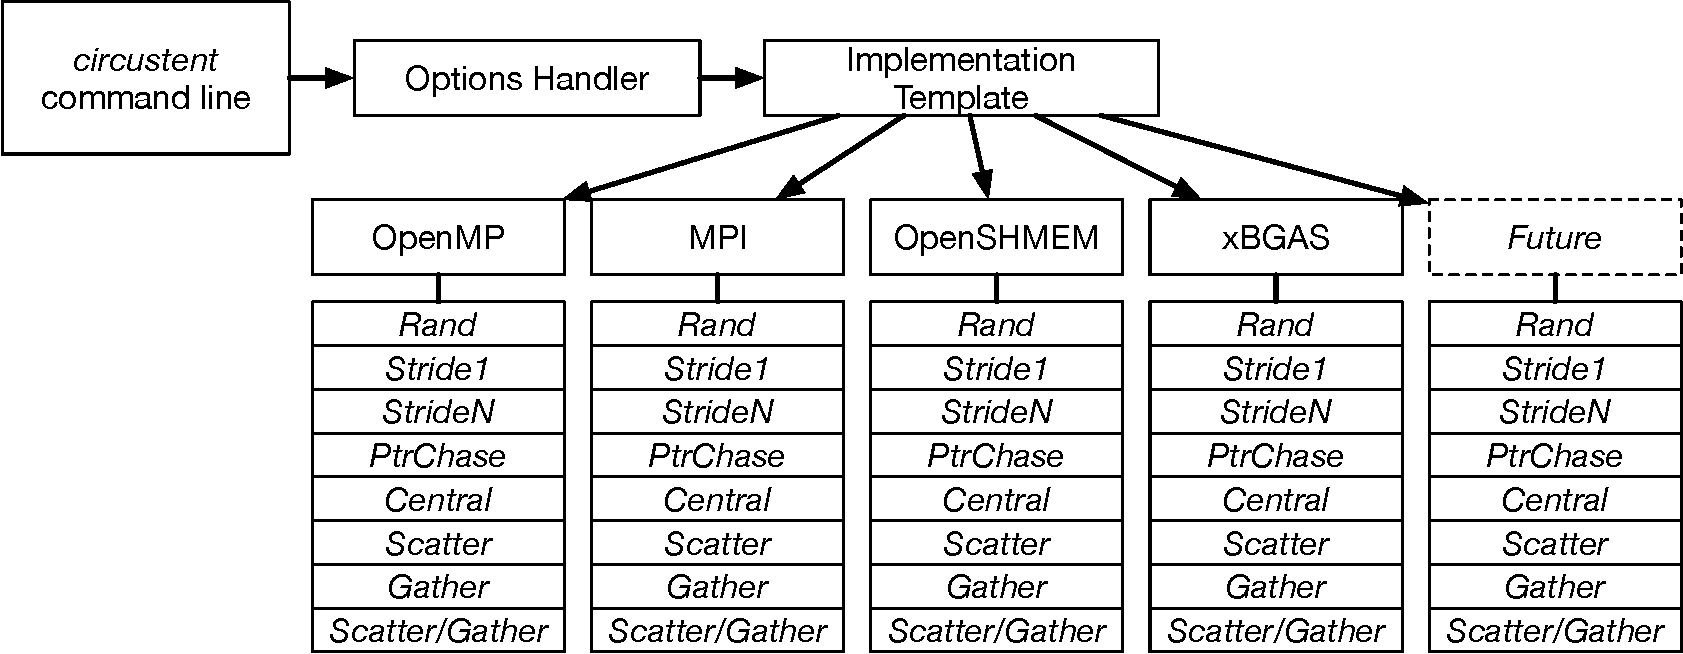
\includegraphics[width=5in]{figures/arch.pdf}
\caption{CircusTent Architecture}
\label{fig:ct_arch}
\end{figure*}

\subsection{Benchmark Overview}
\label{subsec:benchmark_overview}

\subsection{Programming Models}
\label{subsec:programming_models}

\subsection{Algorithms}
\label{subsec:algorithms}

The CircusTent infrastructure contains eight individual benchmark kernels.
Each kernel is described in terms of a generic atomic operation, \textit{AMO}.  
However, each kernel may be implemented using any platform-supported atomic operations.
In the case of this study, we utilize atomic \textit{Add} and atomic \textit{Compare-and-Swap} (CAS) operations to implement each kernel, respectively.  

The first kernel is a basic random access kernel (Algorithm~\ref{alg:1}).
The kernel allocates two array structures.
The \texttt{VAL} array contains a series of values.
The \texttt{IDX} array contains a series of valid indices within the scope of the \texttt{VAL} array.
Prior to the execution of the kernel, the indices are randomly selected and written to the \texttt{IDX} array using a linear congruential randomizer.
For each iteration of the loop, a single \texttt{VAL} array entry is updated using an atomic operation.
In this manner, the random access kernel contains one memory load (\texttt{IDX[i]}) and one atomic operation for each iteration of the loop.
The goal of this kernel is to observe the performance of atomic operations when the platform has a limited ability to cache data for subsequent iterations.  

\begin{algorithm}
\SetAlgoLined
\For{$i\gets0$ \KwTo $iters$ \KwBy $1$}{
AMO(VAL[IDX[i]])
}
\caption{Random Access Kernel}
\label{alg:1}
\end{algorithm}

The second kernel encapsulates a simple, stride-1 kernel (Algorithm~\ref{alg:2}).  
The kernel allocates a single array (\texttt{VAL}) that contains a series of values.  
For each iteration of the loop, the kernel updates a single value in the array in linear fashion using a single atomic operation.
In this manner, a platform may utilize data prefetching and/or caching in order to optimize the access to data members in this kernel in an optimal manner similar in form to dense vectors or matrices.  

\begin{algorithm}
\SetAlgoLined
\For{$i\gets0$ \KwTo $iters$ \KwBy $1$}{
AMO(VAL[i])
}
\caption{Stride-1 Kernel}
\label{alg:2}
\end{algorithm}

The third kernel is similar in form to the second kernel.
In this kernel, we utilize the same \texttt{VAL} array structure as mentioned above, but we permit the user to define the unit stride by which we access the array (Algorithm~\ref{alg:3}).  
For example, if the user seeks to determine what the raw memory bandwidth is of parallel atomics by forcing every access to induce a cache line miss, the stride-n kernel can accomplish this.
Further, for each parallel PE participating in the kernel execution, the starting index is at least \textit{iters} distance from the previous PE. 

\begin{algorithm}
\SetAlgoLined
\For{$i\gets0$ \KwTo $iters$ \KwBy $stride$}{
AMO(ARRAY[i])
}
\caption{Stride-N Kernel}
\label{alg:3}
\end{algorithm}

The fourth

\begin{algorithm}
\SetAlgoLined
\For{$i\gets0$ \KwTo $iters$ \KwBy $1$}{
start = AMO(IDX[start])
}
\caption{Pointer Chase Kernel}
\label{alg:4}
\end{algorithm}

\begin{algorithm}
\SetAlgoLined
\For{$i\gets0$ \KwTo $iters$ \KwBy $1$}{
AMO(ARRAY[0])
}
\caption{Central Kernel}
\label{alg:5}
\end{algorithm}

\begin{algorithm}
\SetAlgoLined
\For{$i\gets0$ \KwTo $iters$ \KwBy $1$}{
dest = AMO(IDX[i+1])\\
val = AMO(ARRAY[i])\\
AMO(ARRAY[dest], val) // ARRAY[dest] = val
}
\caption{Scatter Kernel}
\label{alg:6}
\end{algorithm}

\begin{algorithm}
\SetAlgoLined
\For{$i\gets0$ \KwTo $iters$ \KwBy $1$}{
dest = AMO(IDX[i+1])\\
val = AMO(ARRAY[dest])\\
AMO(ARRAY[i], val) // ARRAY[i] = val
}
\caption{Gather Kernel}
\label{alg:7}
\end{algorithm}

\begin{algorithm}
\SetAlgoLined
\For{$i\gets0$ \KwTo $iters$ \KwBy $1$}{
src = AMO(IDX[i])\\
dest = AMO(IDX[i+1])\\
val = AMO(ARRAY[src])\\
AMO(ARRAY[dest], val) // ARRAY[dest] = val
}
\caption{Scatter/Gather Kernel}
\label{alg:8}
\end{algorithm}

We summarize the number of atomic operations required to perform each kernel in Table~\ref{tab:amodistro}.
However, this may vary depending upon how each platform implements a respective atomic operation.
The CircusTent implementation infrastructure supports the ability to override these defaults for each platform/programming model.    

\begin{table}
  \caption{Atomic Operation Distribution}
  \label{tab:amodistro}
  \begin{tabular}{cc}
    \toprule
    Benchmark&AMOs Per Iteration\\
    \midrule
   Rand & 1\\
   Stride-1 & 1\\
   Stride-N & 1\\
   Pointer Chase & 1\\
   Central & 1\\
   Scatter & 3\\
   Gather & 3\\
   Scatter/Gather & 4\\
  \bottomrule
\end{tabular}
\end{table}

\subsection{Normalizing the Results}
\label{subsec:normalizingtheresults}

Given the native extensibility of CircusTent to support a multitude of programming models and platforms, we seek to develop a normalized metric such that we can compare results across platforms and differing degrees of execution parallelism.
For this, we introduce the \textit{GAMs} metric.  

The \textit{GAMs}, or \textit{billions of atomic operations per second}, metric encapsulates the number of parallel execution elements (\textit{PEs}), the atomic operation algorithmic complexity, and the wall clock execution time in a single metric.
As we see in Equation~\ref{eq:gams}, the metric is a ratio of the total number of atomic operations executed for all parallel parallel execution elements (in billions) across all iterations and the wall clock execution time.
The atomic operation algorithmic complexity is the total number of atomic operations required for a single \textit{PE} to execute a single iteration of the target CircusTent kernel.
This is equivalent to the \textit{AMOs Per Iteration} column in Table~\ref{tab:amodistro}.  

\begin{equation}
\label{eq:gams}
  GAMs = \frac{(PEs \times Iters \times AMOs\_Per\_Iter)/1e^{9}}{time}
\end{equation}


% Benchmark Evaluation
\section{Benchmark Evaluation}
\label{sec:benchmark_evaluation}
% Benchmark Evaluation Section

In order to demonstrate the capabilities of the CircusTent benchmark suite, in this section we conduct an evaluation of atomic memory operations on a variety of different test platforms.
We first introduce our test platforms and briefly describe pertinent details of their underlying architecture in section ~\ref{subsec:platforms}.
We next detail our evaluation methodology in section ~\ref{subsec:methodology}.
Finally, we present and discuss the our evaluation results for each of the CircusTent kernels in section ~\ref{subsec:results}.

\subsection{Platforms}
\label{subsec:platforms}

We evaluate CircusTent across a total of fourteen different platforms.
The platforms encompass a variety of different device classes/architectures that include embedded, laptop, desktop, server, and petascale class supercomputers.
Further, the processors utilized encompass a variety of different instruction set architectures from Intel, AMD, and ARM.
These systems feature both single and dual socket systems whose processors have varied core counts and clock speeds.
Further, the complexity of these system's memory subsystem and cache hierarchy are similar varied.

However, using CircusTent and our normalized GAMs metric, we are able to directly compare the performance of these memory hierarchies with respect to atomic operations in a variety of different scenarios. (using memory access patterns common in...).
Table ~\ref{tab:benchsys} provides an overview of our test platforms specifications wherein each system is denoted by its processor.
In addition, we also provide a brief description of each platform in the list below.
In particular, we detail the implementation of each platform's cache hierarchy as this directly correlates to its shared memory performance. 

\begin{table*}
\caption{Benchmark System Configurations}
\label{tab:benchsys}
\begin{tabular}{ccccp{15mm}ccp{16mm}c}
\toprule
System&Clock Frequency&Cores / Socket&Total Sockets&LLC Size\newline~/ Socket&Total Memory&Array Size&Operating\newline System&Compiler\\
\midrule
Cortex-A53      & 1.40Ghz & 4  & 1 & 64KiB  & 512MiB & 256MiB  & Ubuntu\newline 18.04 4.15.0 & GCC 7.4.0\\
Cortex-A72      & 1.50Ghz & 4  & 1 & 1MiB   & 4GiB & 256MiB  & Debian\newline 10.1 4.19.75 & GCC 8.3.0\\
Ryzen V1605B    & 1.58Ghz & 4  & 1 & 4MiB    & 32GiB & 15GiB & Ubuntu\newline 19.04 5.2.10&GCC 8.3.0\\
Opteron 4130    & 2.60Ghz & 4  & 2 & 6MiB   & 64GiB & 15GiB & Centos7\newline 3.10.0&GCC 8.3.1\\
Core i5-3210M   & 2.50Ghz & 2  & 1 & 3MiB   & 4GiB & 256MiB & macOS\newline 10.13.6&clang 9.1.0\\
Core i7-3930K   & 3.20Ghz & 6  & 1 & 12MiB  & 64GiB & 15GiB & Linux Mint\newline 18.3 4.15.0&GCC 5.4.0\\
Core i7-4980HQ  & 2.80Ghz & 4  & 1 & 6MiB L3 +\newline 128MiB L4 & 16GiB & 15GiB & macOS\newline 10.15.3&GCC 9.2.0\\
Xeon Phi 7250   & 1.40Ghz & 68 & 1 & 16GiB \newline MCDRAM & 96GiB & 15GiB & SLES\newline 4.12.14&GCC 8.3.0\\
Xeon E5620      & 2.40Ghz & 4  & 2 & 12MiB & 48GiB & 15GiB & Ubuntu\newline 16.04 4.4.0&GCC 5.4.0\\
Xeon X5650      & 2.67Ghz & 6  & 2 & 12MiB & 64GiB & 15GiB & Ubuntu\newline 18.04 4.15.0&GCC 7.5.0\\
Xeon E5-2620 v3 & 2.40Ghz & 6  & 1 & 15MiB & 64GiB & 15GiB & Ubuntu\newline 16.04 4.4.0&GCC 5.4.0\\
Xeon E5-2670 v2 & 2.50Ghz & 10 & 2 & 25MiB & 64GiB & 15GiB & Centos7\newline 3.10.0&GCC 7.3.0\\
Xeon E5-2695 v4 & 2.10Ghz & 18 & 2 & 45MiB & 192GiB & 15GiB & Centos7\newline 3.10.0&GCC 7.3.0\\
Xeon E5-2698 v3 & 2.30Ghz & 16 & 2 & 40MiB & 128GiB & 15GiB & SLES\newline 4.12.14&GCC 8.3.0\\
\bottomrule
\end{tabular}
\end{table*}

\todo[inline]{Double check system specs and array sizes with John}

\subsection{Methodology}
\label{subsec:methodology}

Consistent with previous studies, we focus on evaluating the CircusTent suite in a shared-memory environment in this work\cite{}.
In order to do so, we execute each of the CircusTent kernels, detailed in section ~\ref{subsec:algorithms}, on the test platforms introduced above using the OpenMP-based CircusTent benchmark implementation. For each kernel, we conduct trials using both the atomic \textit{Add} and \textit{Compare-and-Swap} implementations.
For both versions, 64-bit operands are used throughout the evaluation to prevent any inconsistencies.
For the StrideN kernel, a uniform unit stride size of 9 is utilized for each trial.

We collect performance results on each platform.
In order to eliminate any performance variability associated with simultaneous multithreading (SMT), we vary the thread count from a single thread up to one thread per physical core for each platform.
Moreover, to better simulate real-world behavior, we allow the operating system and programming model to perform the mapping of threads to processor cores.

Where feasible, a uniform size of approximately 15 GiB is utilized for the \texttt{VAL} array on each platform. For the Cortex A-53, Cortex A-72, and Core i5-3210M systems, wherein physical memory limitations make this configuration impractical, a size of 256 MiB is utilized instead.
In order to generate sufficient runtime such that the benchmark's behavior normalizes, twenty million iterations are run as part of each trial conducted for each kernel.

\todo[inline]{Add previous shared-memory references}

\subsection{Results}
\label{subsec:results}

\begin{figure}[!t]
\centering
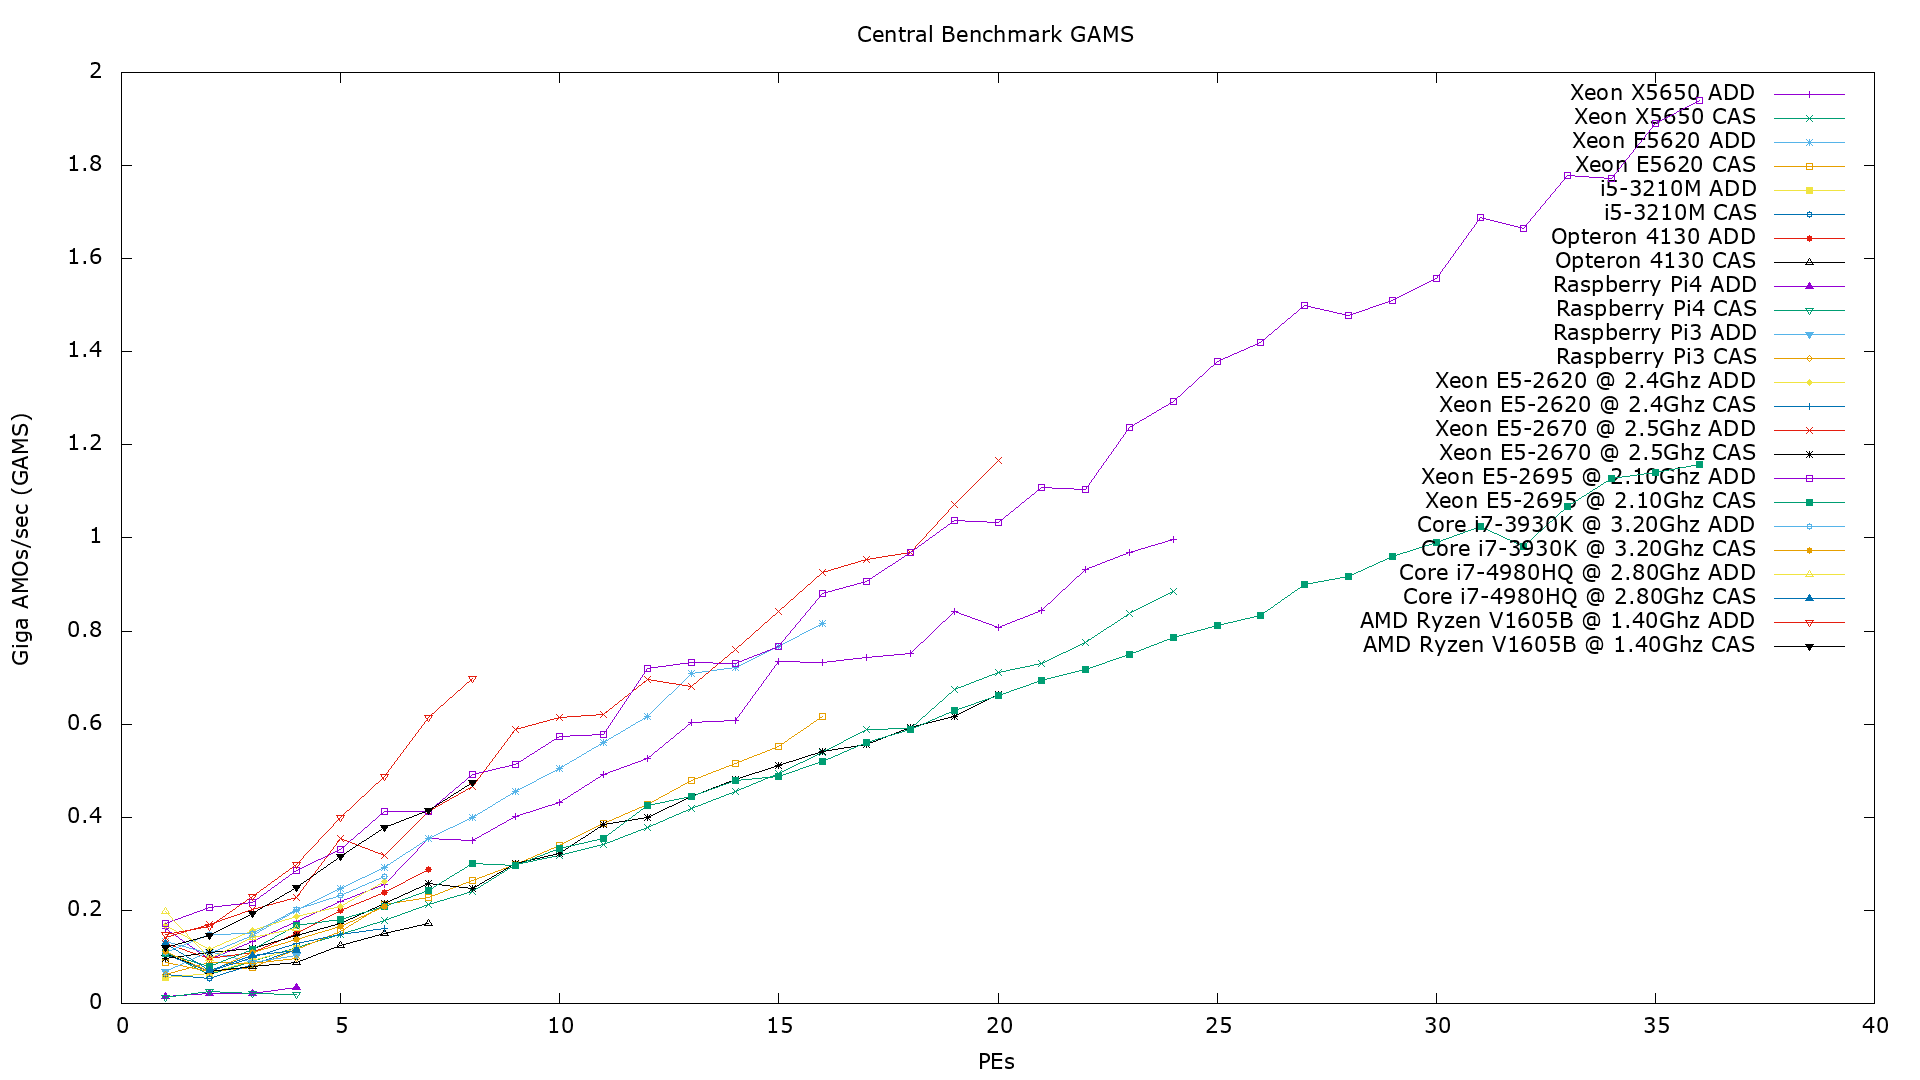
\includegraphics[width=3.5in]{figures/CENTRAL_GAMS.png}
\caption{Central Benchmark GAMS}
\label{fig:central_gams}
\end{figure}

\begin{figure}[!t]
\centering
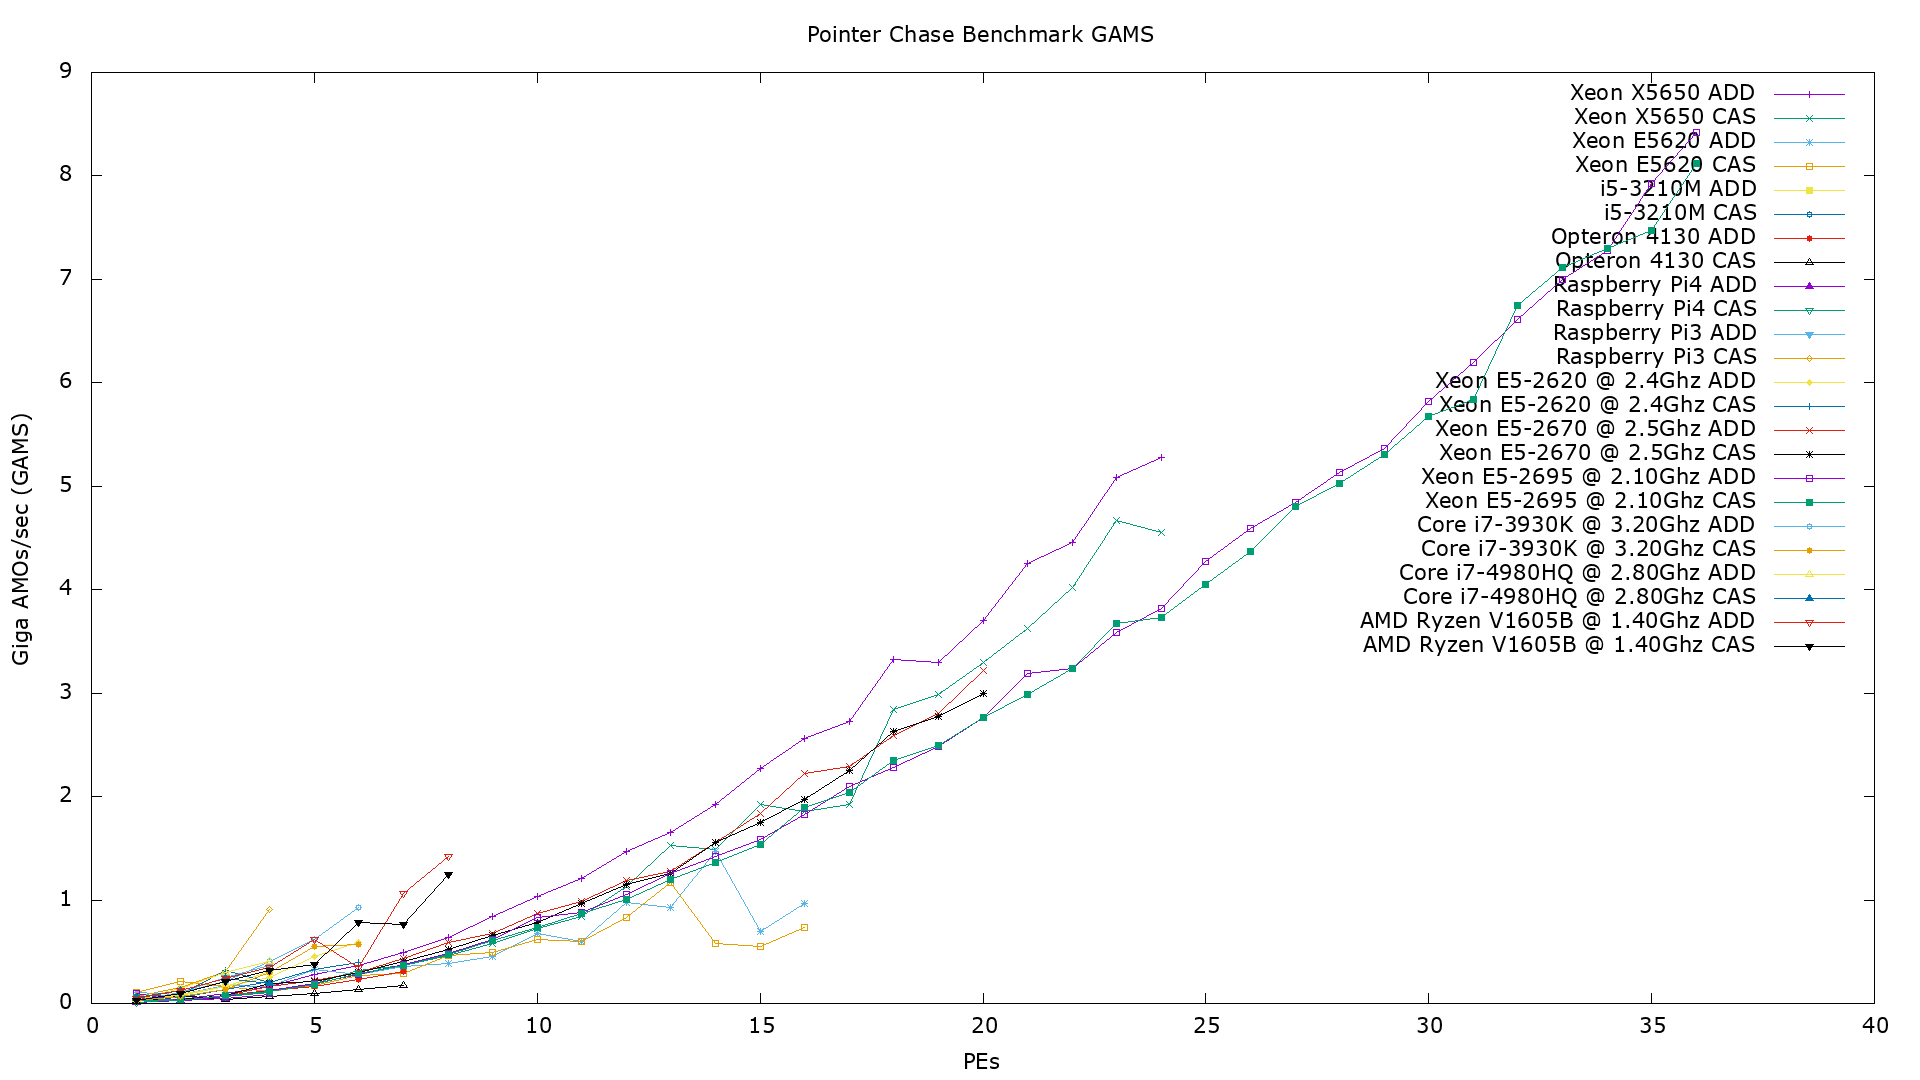
\includegraphics[width=3.5in]{figures/PTRCHASE_GAMS.png}
\caption{Pointer Chase Benchmark GAMS}
\label{fig:ptrchase_gams}
\end{figure}

\begin{figure}[!t]
\centering
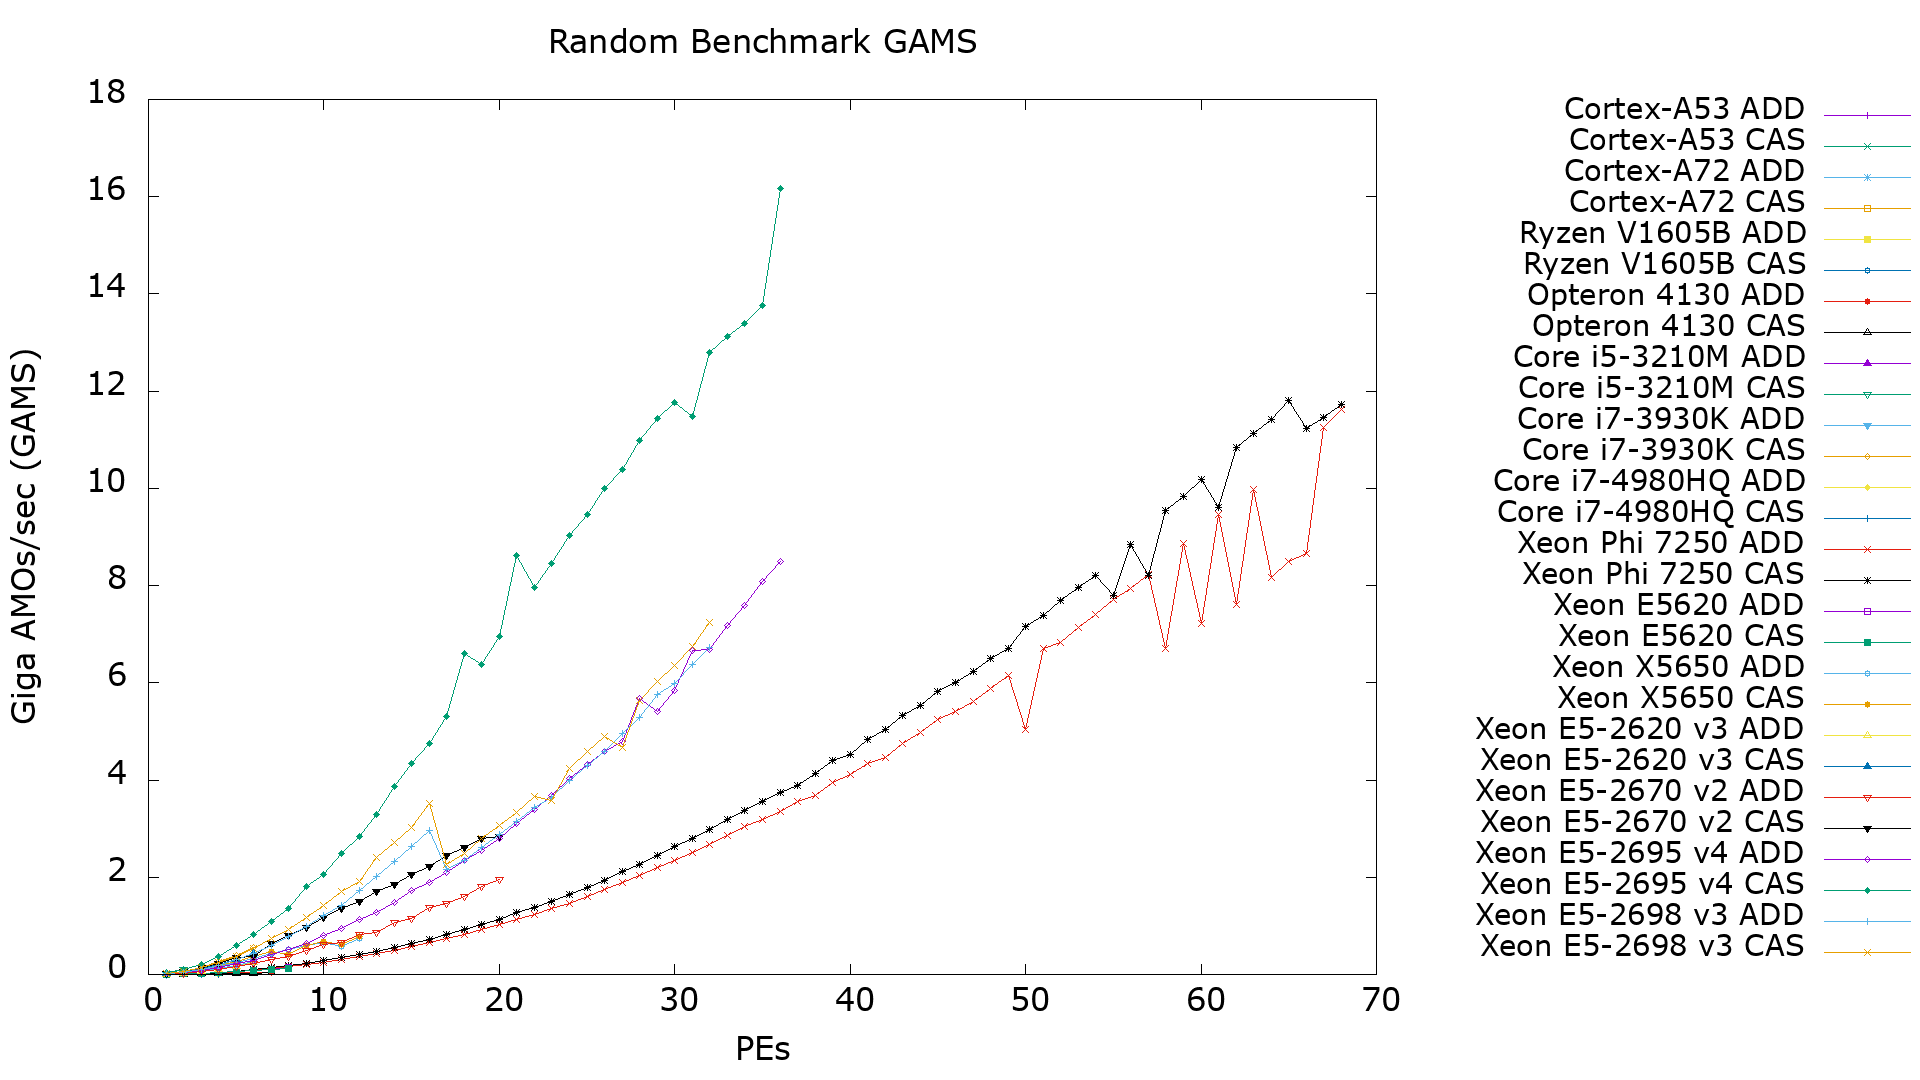
\includegraphics[width=3.5in]{figures/RAND_GAMS.png}
\caption{Random Benchmark GAMS}
\label{fig:rand_gams}
\end{figure}

\begin{figure}[!t]
\centering
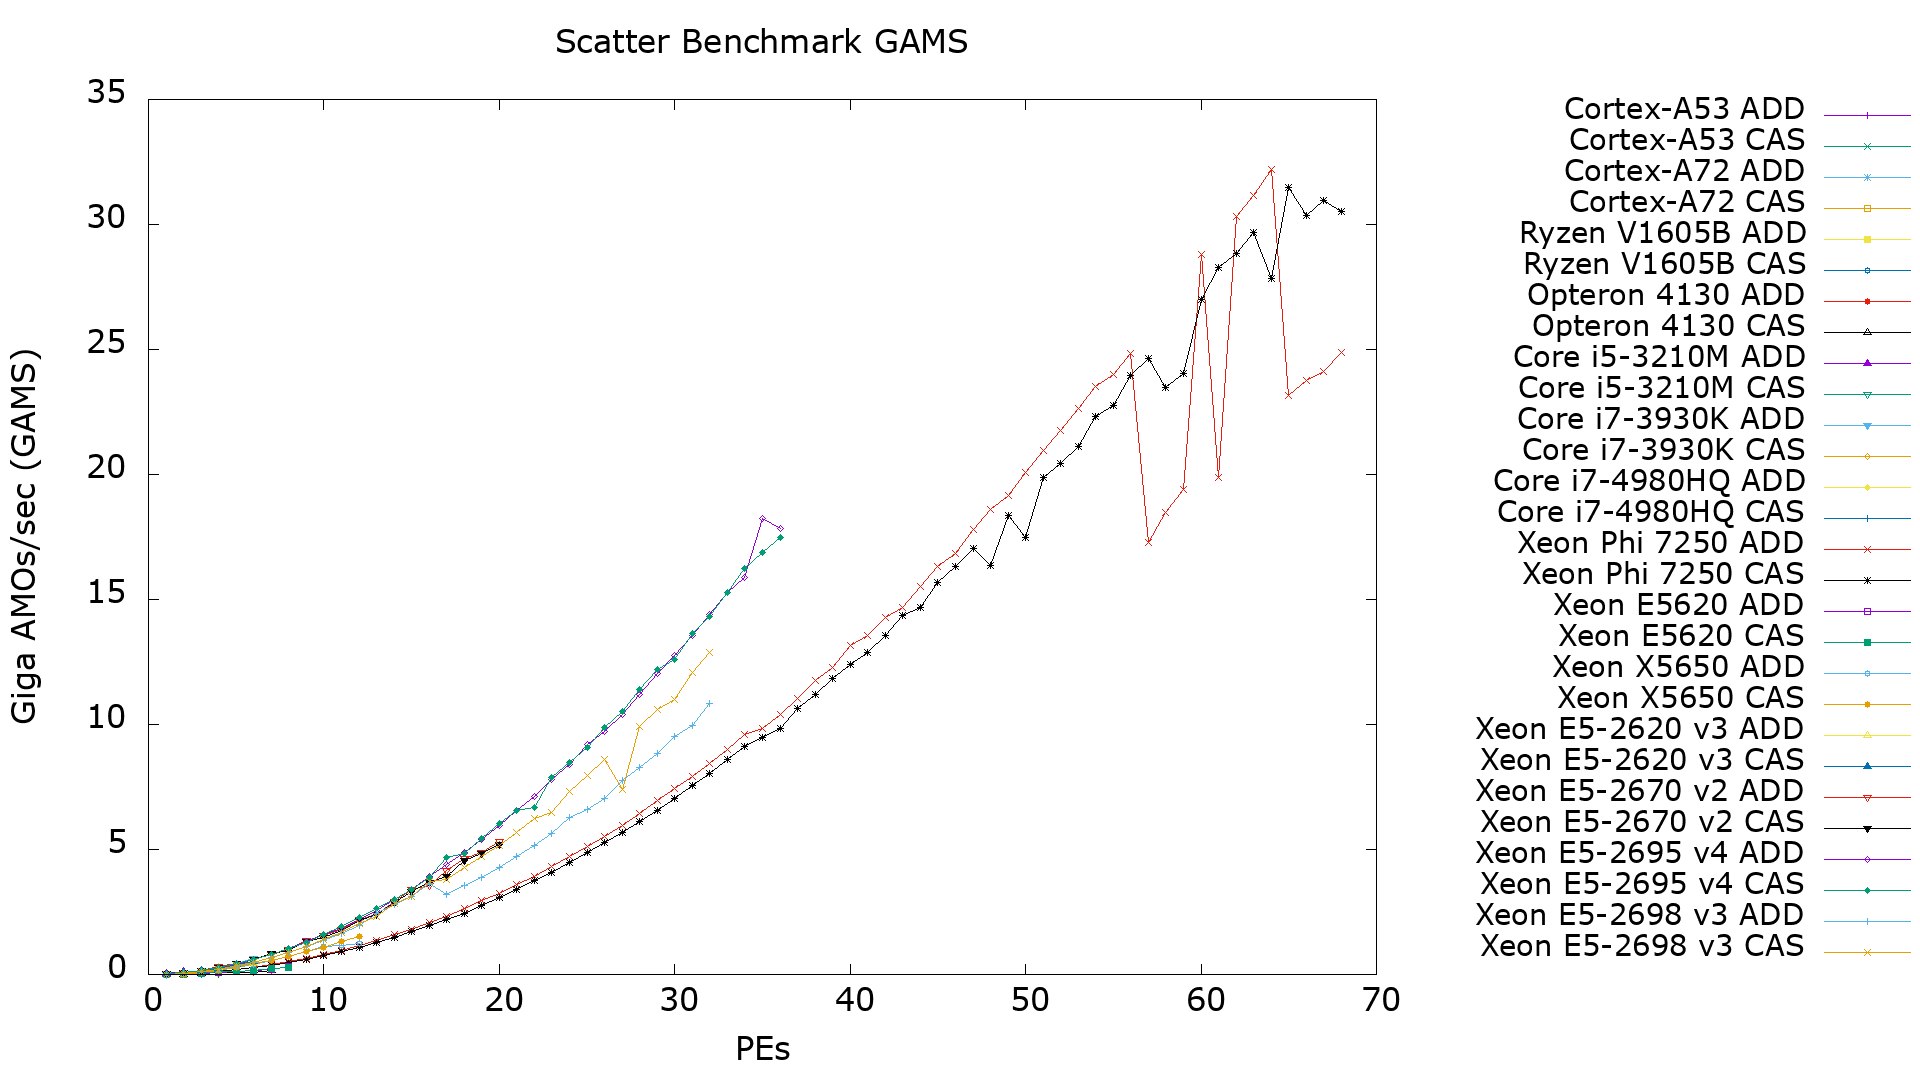
\includegraphics[width=3.5in]{figures/SCATTER_GAMS.png}
\caption{Scatter Benchmark GAMS}
\label{fig:scatter_gams}
\end{figure}

\begin{figure}[!t]
\centering
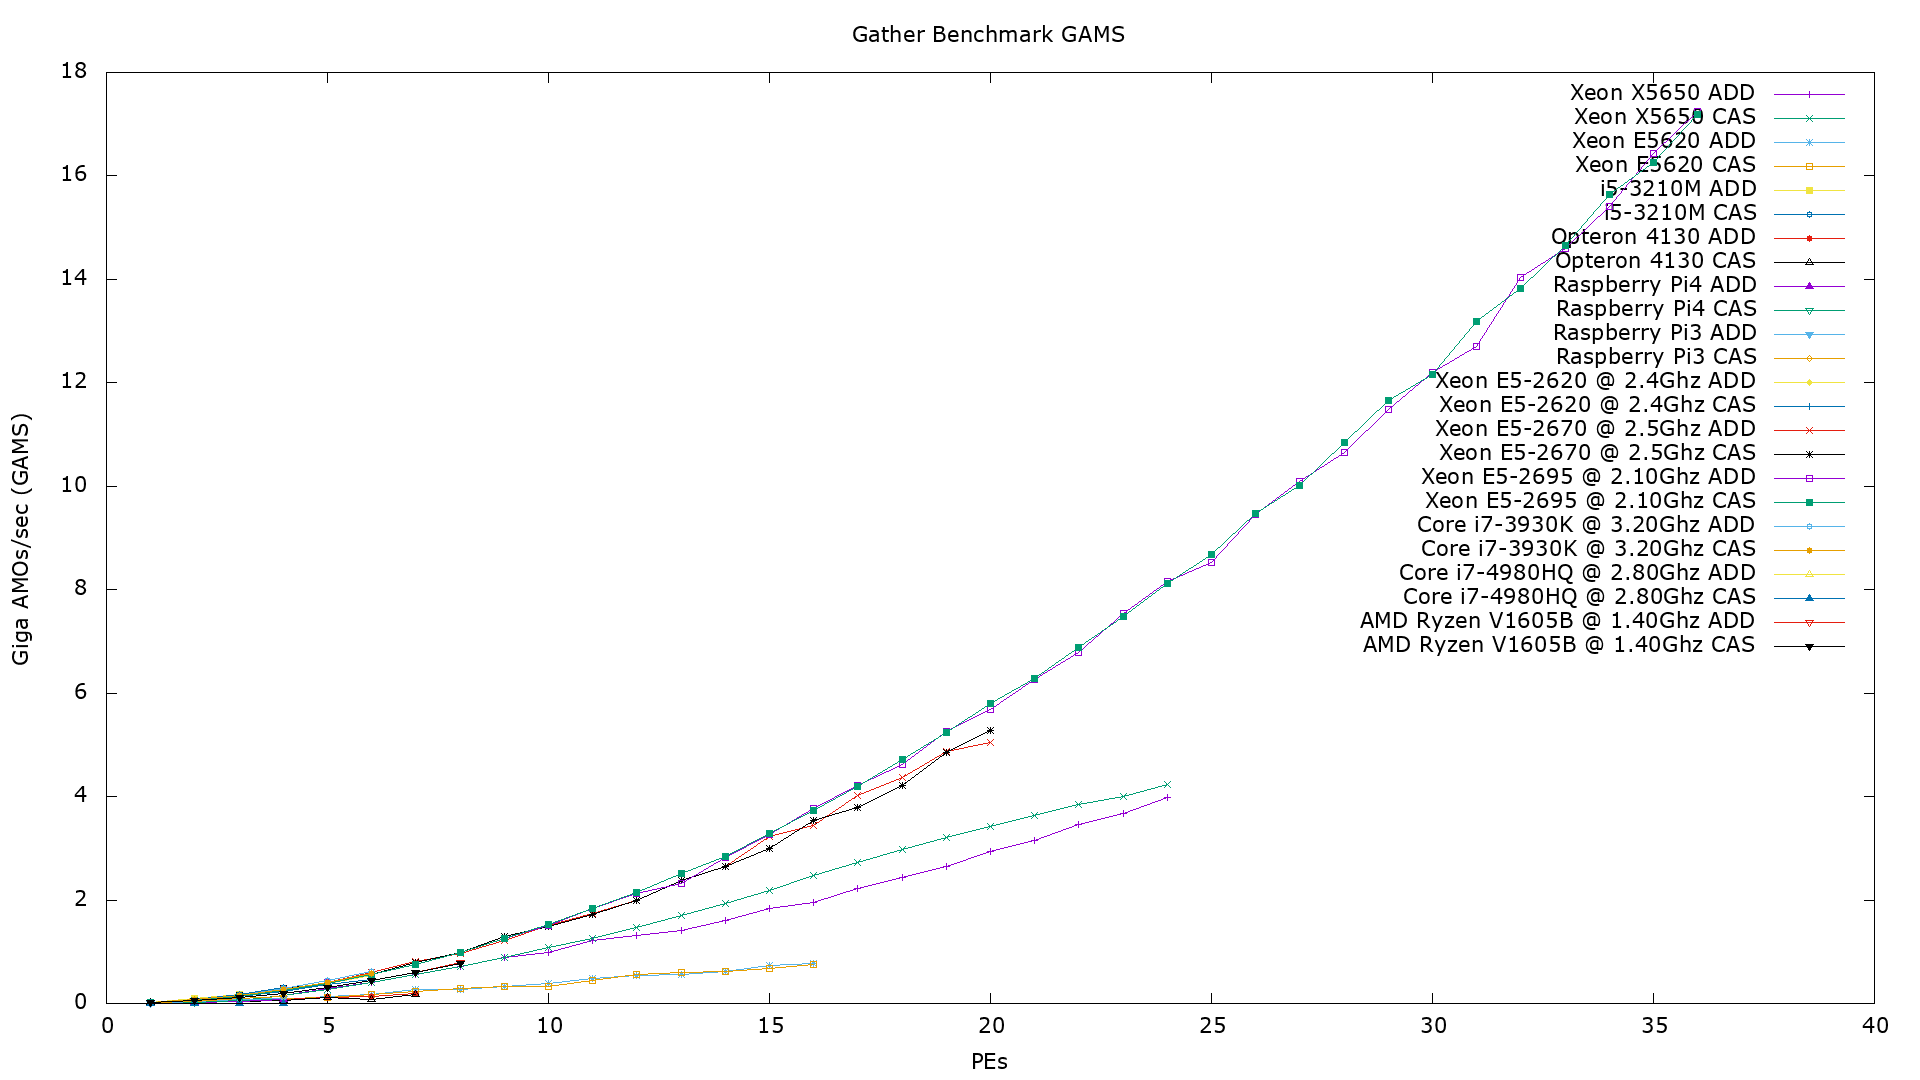
\includegraphics[width=3.5in]{figures/GATHER_GAMS.png}
\caption{Gather Benchmark GAMS}
\label{fig:gather_gams}
\end{figure}

\begin{figure}[!t]
\centering
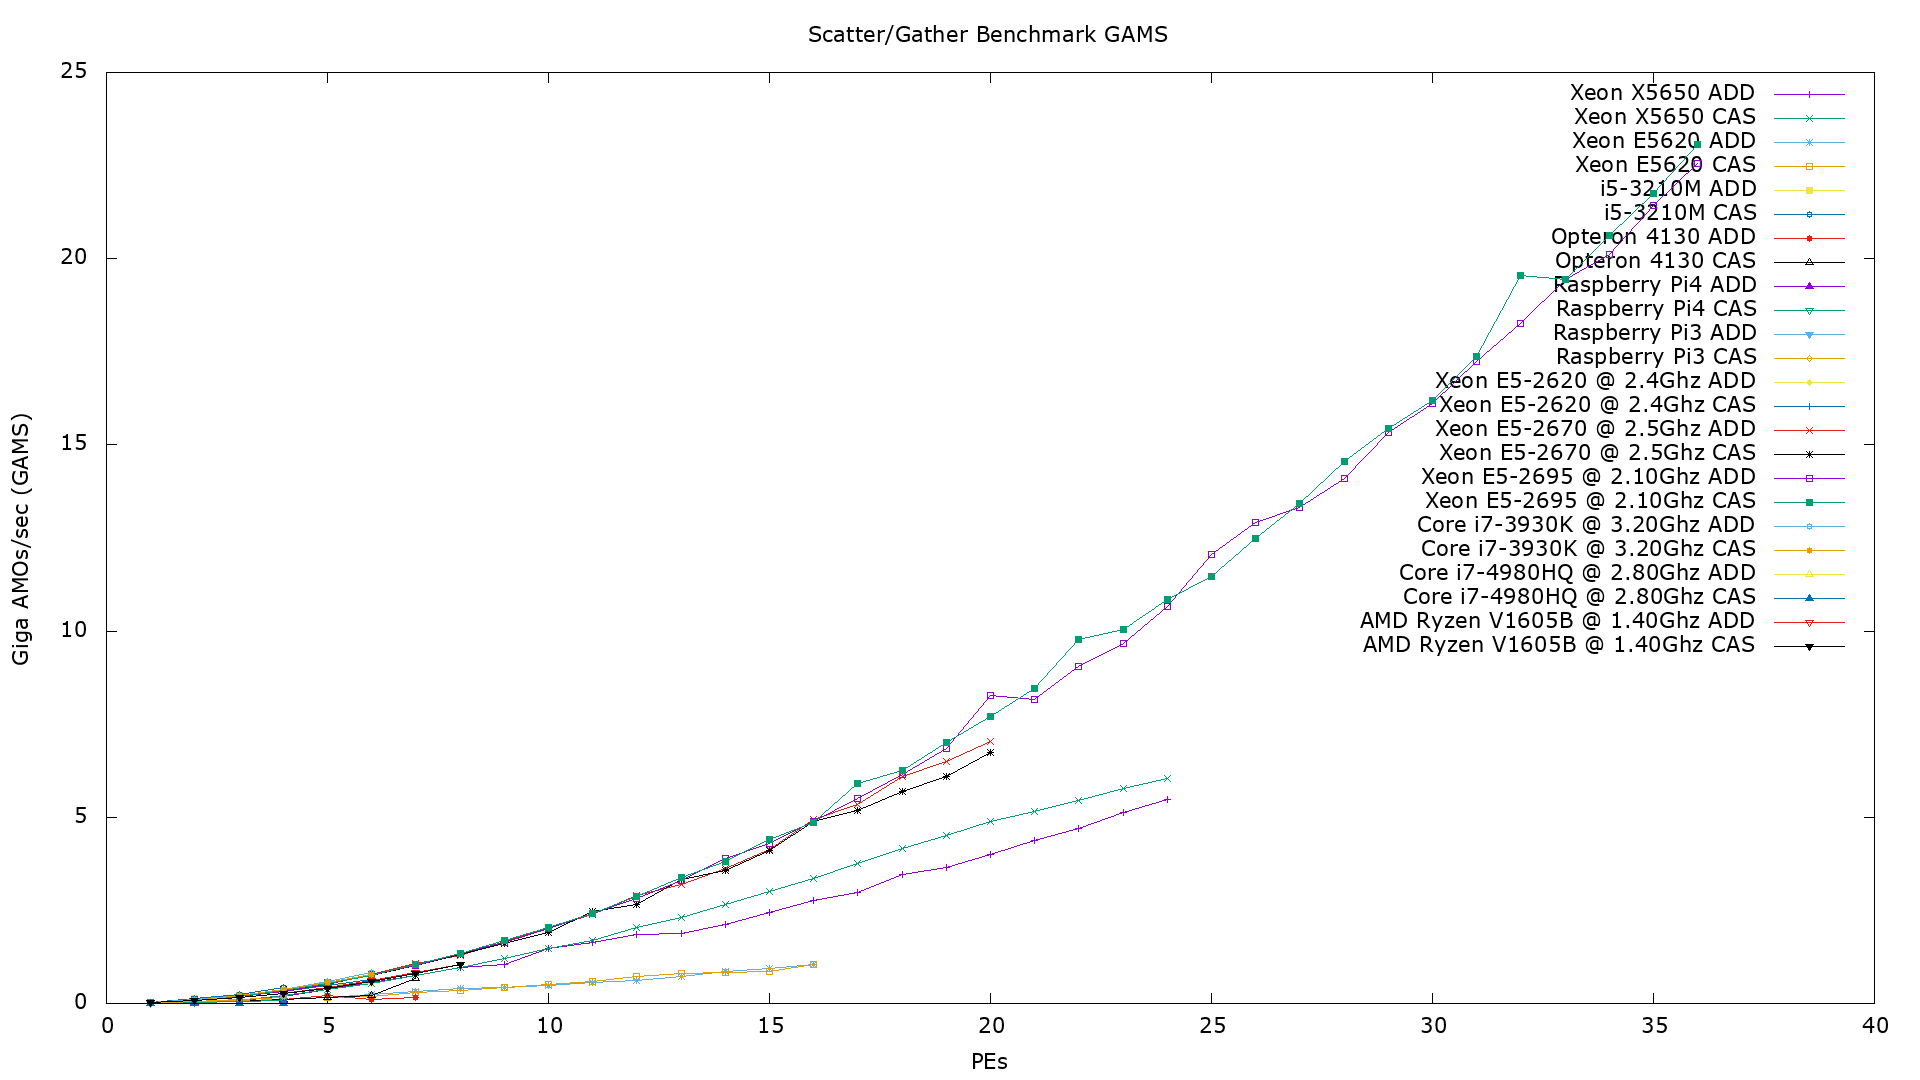
\includegraphics[width=3.5in]{figures/SG_GAMS.png}
\caption{Scatter/Gather Benchmark GAMS}
\label{fig:sg_gams}
\end{figure}

\begin{figure}[!t]
\centering
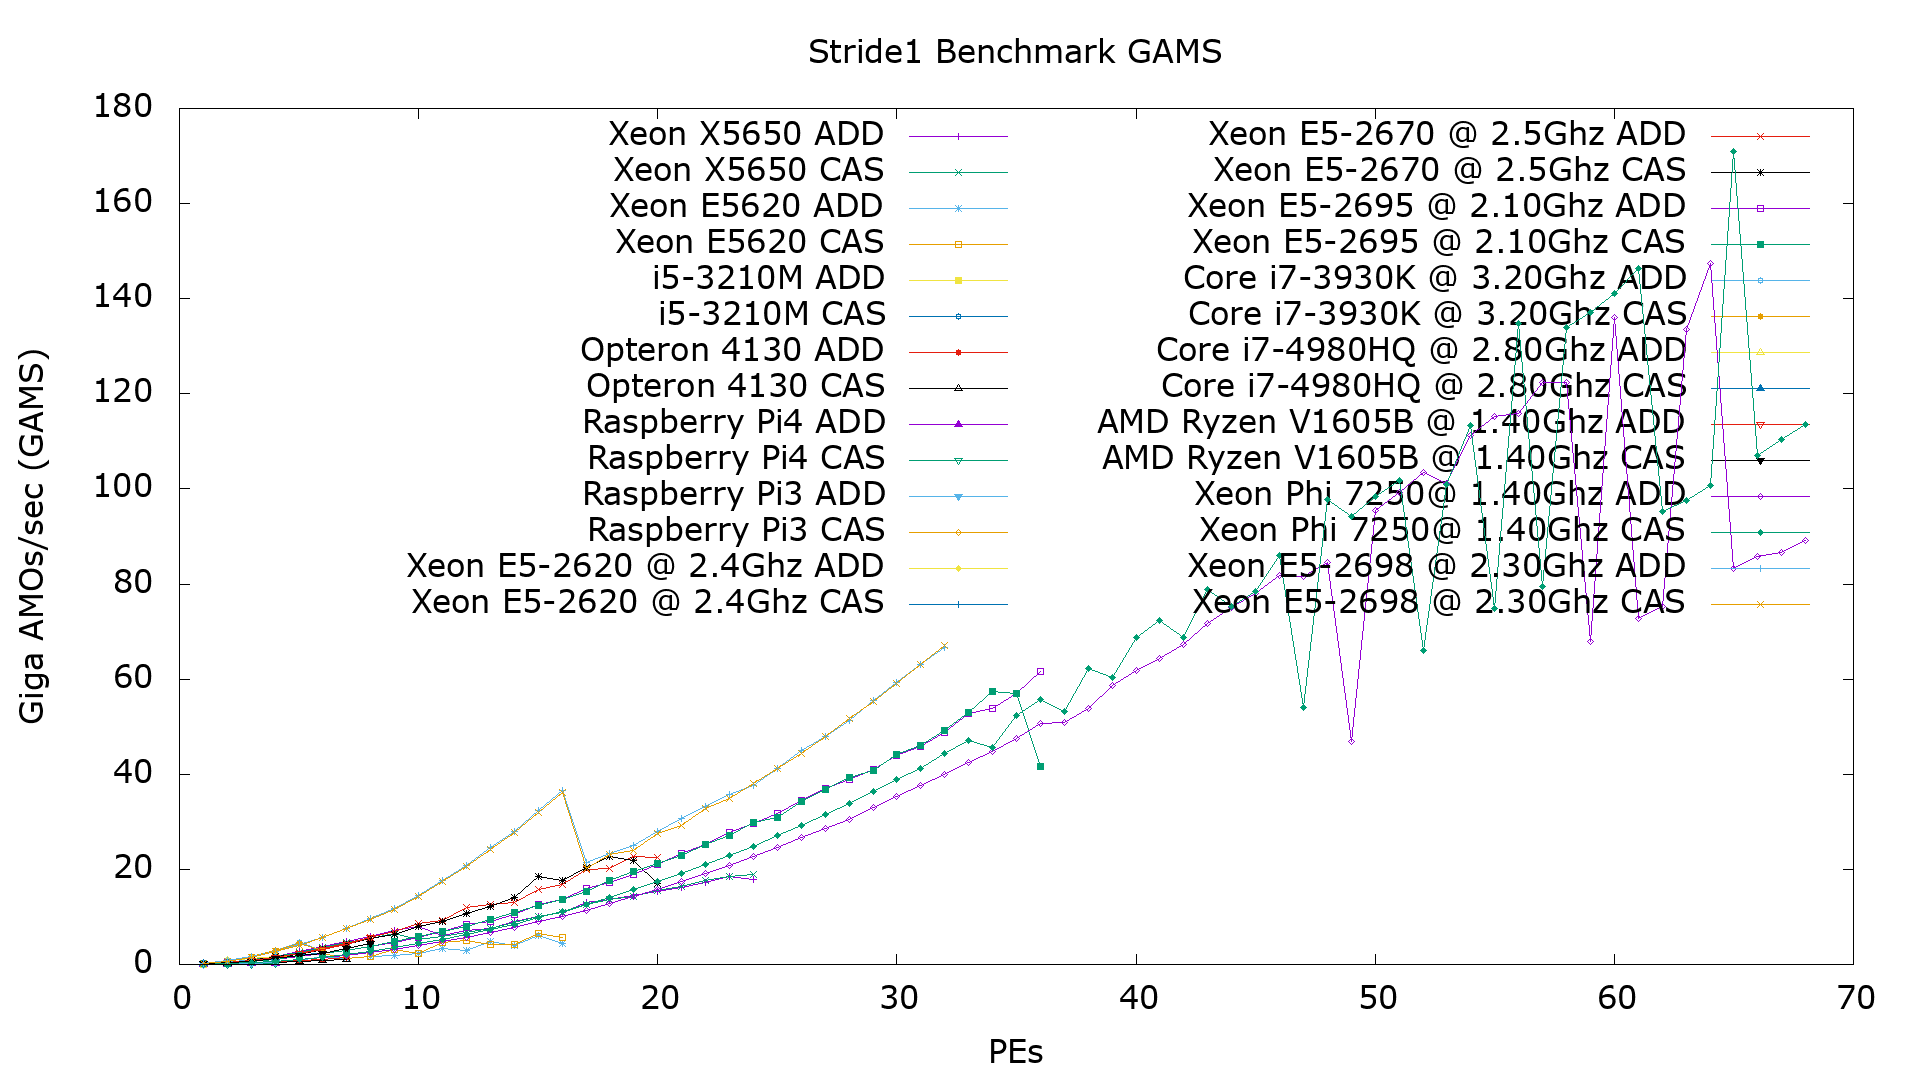
\includegraphics[width=3.5in]{figures/STRIDE1_GAMS.png}
\caption{Stride-1 Benchmark GAMS}
\label{fig:s1_gams}
\end{figure}

\begin{figure}[!t]
\centering
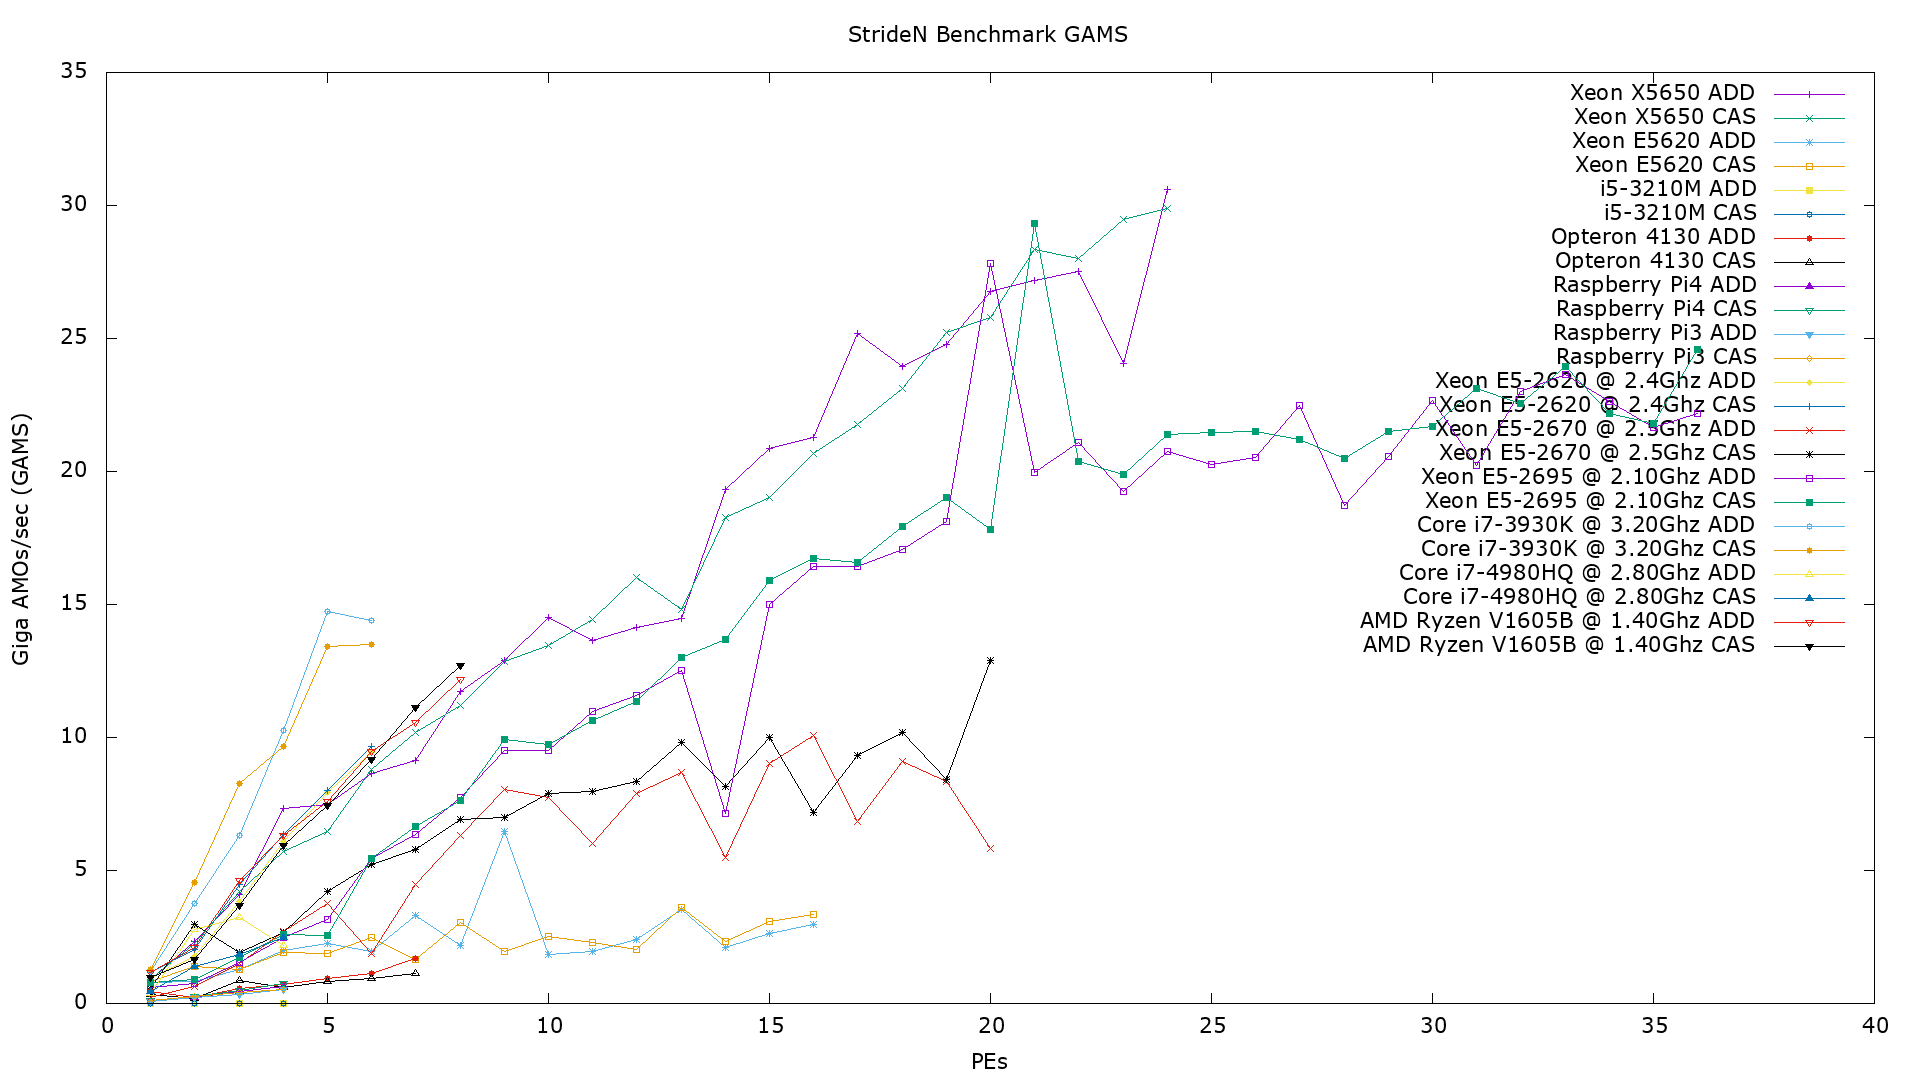
\includegraphics[width=3.5in]{figures/STRIDEN_GAMS.png}
\caption{Stride-N Benchmark GAMS}
\label{fig:sn_gams}
\end{figure}


% Conclusions
\section{Conclusions}
\label{sec:conclusions}
% Conclusions Section

The performance of atomic operations plays a critical role in the scalability of existing systems.
As the degree of heterogeneity and complexity of memory hierarchies in future systems increases, this trend can only be expected to continue, if not intensify.
However, to the best of our knowledge, a comprehensive methodology for measuring the performance of memory subsystems with respect to atomic operations has yet to emerge.

In this work, we introduced the open source CircusTent benchmark suite to fill this void.
Orthogonal to previous works, CircusTent measures the performance of disparate architectures in a generalized manner using common parallel programming paradigms.
Herein, we showcased the modular design of CircusTent that enables native extensibilty for future refinements and additional programming models.
We explored our current backend implementations, designed for both physically shared and distributed shared memory systems, built upon the OpenMP, MPI, and OpenSHMEM programming models as well the xBGAS microarchitecture extension.
We also detailed the eight kernels, designed to replicate atomic memory access patterns common in high-performance computing applications, that constitute the CircusTent suite.

Finally, utilizing our OpenMP backend, we performed an extensive evaluation of CircusTent across fourteen diverse test platforms.
Through the use of our normalized \textit{GAMs} metric, we were able to directly measure and compare the performance of these disparate systems.
In line with previous work and conventional wisdom, our results showed that both the memory access patterns of a given application and the cache organization of a target system significantly affect its performance with respect to atomic operations.
However, our evaluation also revealed some new insights and diverged from our expectations with regard to several of our test platforms.

We feel our evaluation clearly demonstrates the capabilities and value of the CircusTent benchmark suite.
As such, we believe that CircusTent will prove to be a useful tool that aids in both the benchmarking of existing systems as well as the design and prototyping of future systems.

% Future Work
\section{Future Work}
\label{sec:future_work}
% Future Work Section

Although the current CircusTent infrastructure supports a number of modern programming models, we would like to further expand this set of models to better support heterogeneous platforms that include diverse components such as GPUs and FPGAs.
This will require adding support for the OpenMP \textit{target} construct and/or inclusion of additional backends such as OpenACC or CUDA-based implementations.
Alternatively, a more holistic approach could be applied through integration of a modern heterogeneous compilation and runtime infrastructure such as SYCL~\cite{10.1145/3204919.3204930}.  

In addition to the aforementioned heterogeneous system infrastructure, we also seek to expand our benchmark evaluation to include distributed memory platforms and programming models.
Given the current support for MPI and OpenSHMEM, it would be advantageous to execute CircusTent on a variety of interconnects (Infiniband, Cray Aries, Ethernet) at scale in order to derive the performance parameters of atomic memory operations for large-scale system deployments.   

Finally, as parallel programming models continue to evolve and adapt to new system architectures, we will continually update the current CircusTent backend implementations to exploit the latest in programming model optimizations.
Further, we fully expect to continue developing new programming model backends for CircusTent in order to evaluate additional models for future scalable systems.  

\begin{acks}
Research reported in this publication was supported by the U.S. Department of Defense
under Contract FA8075$-$14$-$D$-$0002.
\end{acks}

%---- END CTPAPER

%%
%% The next two lines define the bibliography style to be used, and
%% the bibliography file.
\bibliographystyle{ACM-Reference-Format}
\bibliography{sample-base}

\end{document}
\endinput
%%
%% End of file `sample-sigconf.tex'.
